\chapter{SYSTEM DEMONSTRATION AND OPERATIONAL WALKTHROUGH}

\section{CivicTwin Operations Center Interface Overview}
The CivicTwin user interface is implemented as a single-page web geospatial command application developed using React 18, Vite, and Leaflet GIS. The dashboard is tailored specifically for municipal public works directors, ward engineers, and emergency disaster response coordinators.

Figure~\ref{fig:ui_dashboard} illustrates the primary operational view of the CivicTwin Operations Center running in a standard web browser.

\begin{figure}[h!]
\centering
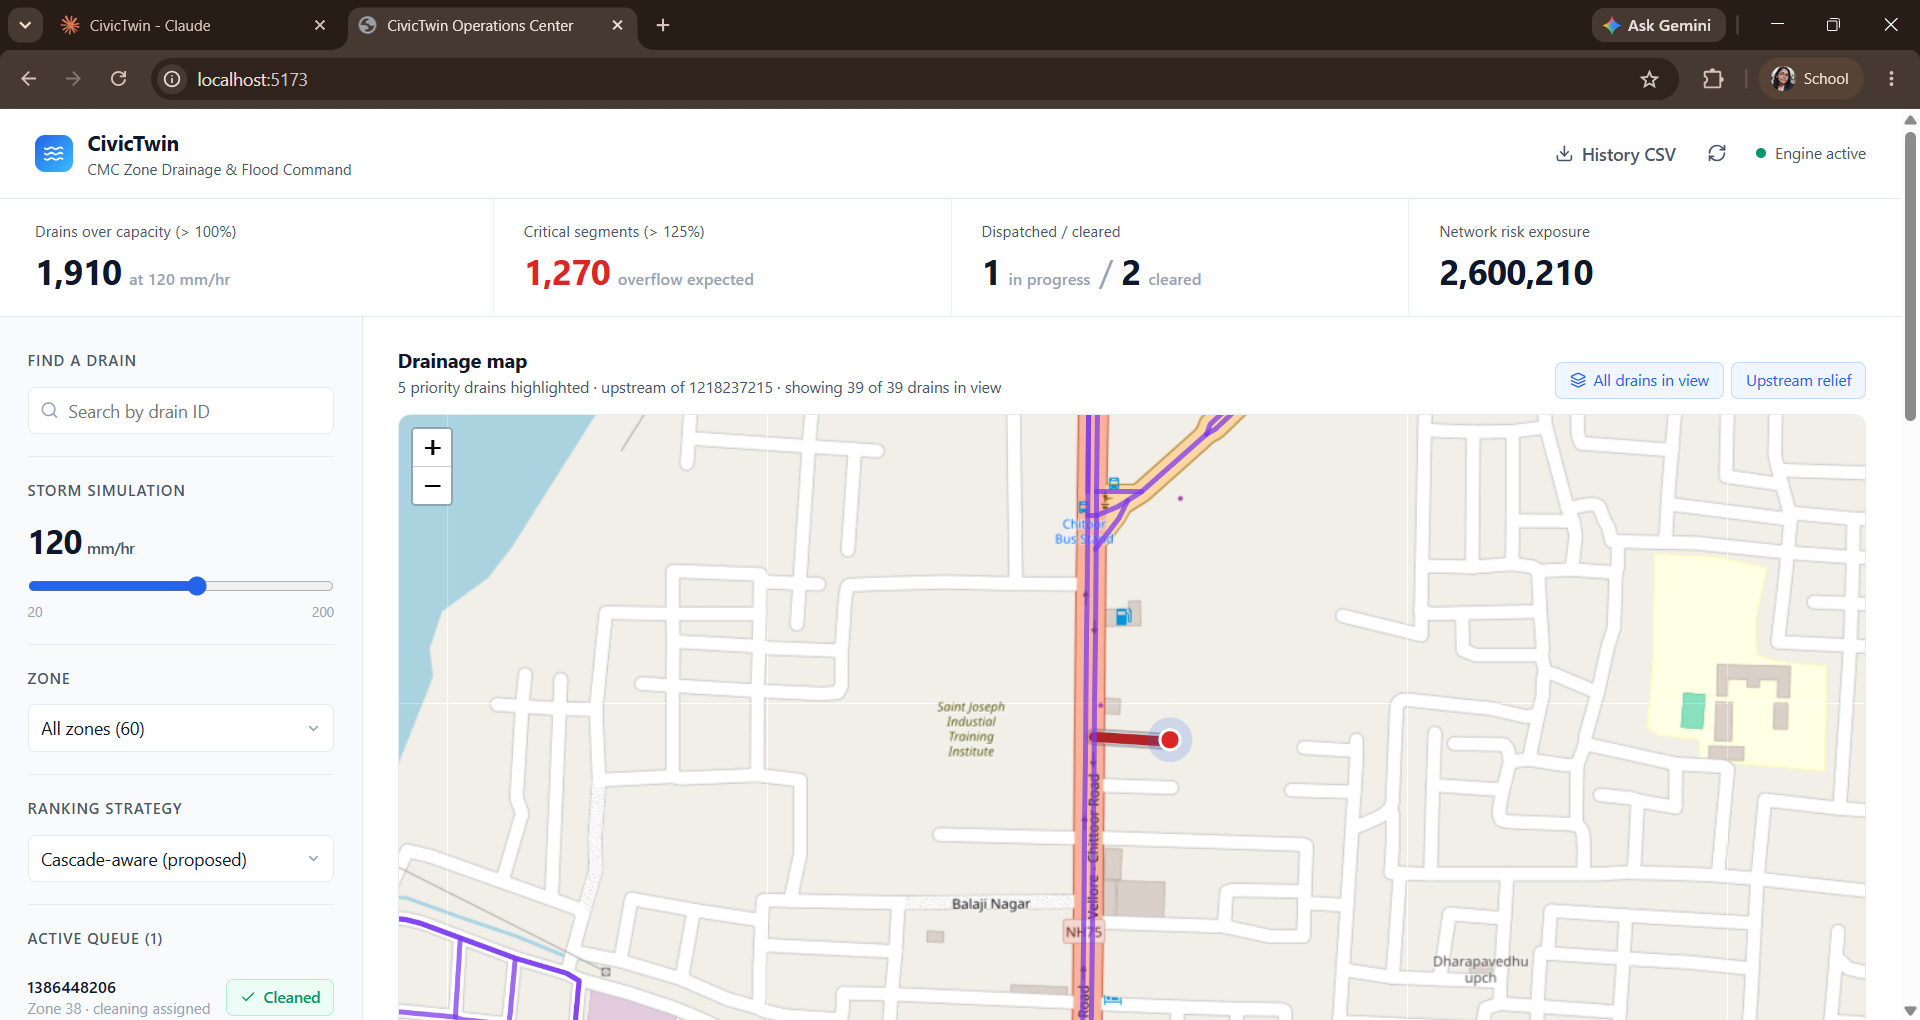
\includegraphics[width=0.98\textwidth]{figures/ui_map_dashboard.png}
\caption{CivicTwin Operations Center Command Dashboard and Geospatial Map}
\label{fig:ui_dashboard}
\end{figure}

The dashboard interface is structured into three integrated functional panels:
\begin{enumerate}
    \item \textbf{Top Executive KPI Banner:} Provides real-time macro-level network indicators, including:
    \begin{itemize}
        \item \textbf{Drains Over Capacity ($> 100\%$):} Total count of conduits experiencing hydraulic overload under current storm settings (e.g., 1,910 segments at 120~mm/hr).
        \item \textbf{Critical Segments ($> 125\%$):} Conduits experiencing severe surcharge where surface street inundation is active (e.g., 1,270 segments).
        \item \textbf{Dispatched / Cleared Status:} Live operational count of work crews actively engaged in the field versus cleared segments (e.g., 1 In-Progress, 2 Cleared).
        \item \textbf{Network Risk Exposure:} The aggregate systemic vulnerability metric ($E_{\text{net}} = 2{,}600{,}210$), dynamically updated as desilting actions are completed.
    \end{itemize}
    \item \textbf{Left Control Sidebar:} Houses administrative filtering and simulation controls, including a text search input for specific conduit IDs, an interactive storm simulation slider ranging from 20 to 200~mm/hr, a zone dropdown selector spanning all 60 municipal clusters, a strategy selection selector, and the active in-progress dispatch queue.
    \item \textbf{Central Geospatial Map Viewport:} An interactive OpenStreetMap vector canvas displaying drainage lines, flow paths, topological junctions, and localized surcharge heatmaps.
\end{enumerate}

\section{Interactive Geospatial Map and Dynamic Viewport Rendering}
Rendering nearly 14,000 multi-point vector polylines simultaneously inside a client browser canvas can degrade rendering performance and frame rates. CivicTwin resolves this via a dynamic bounding-box viewport culling algorithm. As an operator pans or zooms across Vellore Corporation, the map container detects the bounding coordinates:
\begin{equation}
\text{BBox} = \big[\phi_{\min},~\lambda_{\min},~\phi_{\max},~\lambda_{\max}\big]
\end{equation}
The client queries conduits whose spatial bounding box intersects the active viewport, applying zoom-dependent density caps:
\begin{equation}
N_{\text{render}}(\text{zoom}) = \begin{cases}
600 \text{ conduits}, & \text{if zoom} < 14 \\
1{,}000 \text{ conduits}, & \text{if } 14 \le \text{zoom} < 15 \\
1{,}500 \text{ conduits}, & \text{if zoom} \ge 15
\end{cases}
\end{equation}

Conduit vector segments are rendered with semantic color codes representing operational states:
\begin{itemize}
    \item \textbf{Red (\#dc2626):} Critical threat tier ($U > 125\%$), indicating severe localized overflow.
    \item \textbf{Orange (\#f59e0b):} High threat tier ($80\% < U \le 125\%$), indicating near-capacity conditions.
    \item \textbf{Green (\#10b981):} Low threat tier ($U \le 80\%$), indicating safe conveyance.
    \item \textbf{Slate Blue (\#64748b):} Active conduit currently \texttt{IN\_PROGRESS}.
    \item \textbf{Light Grey (\#cbd5e1):} Cleared conduit (\texttt{CLEARED}).
    \item \textbf{Purple (\#7c3aed):} Upstream relief trace, visually highlighting all tributary ancestor channels relieved when a specific conduit is selected.
\end{itemize}

\section{Priority Dispatch Table and Live Surcharge Metrics}
Beneath the geospatial map, the Operations Center renders the dynamic \textbf{Priority Drains Table}, as shown in Figure~\ref{fig:ui_table}.

\begin{figure}[h!]
\centering
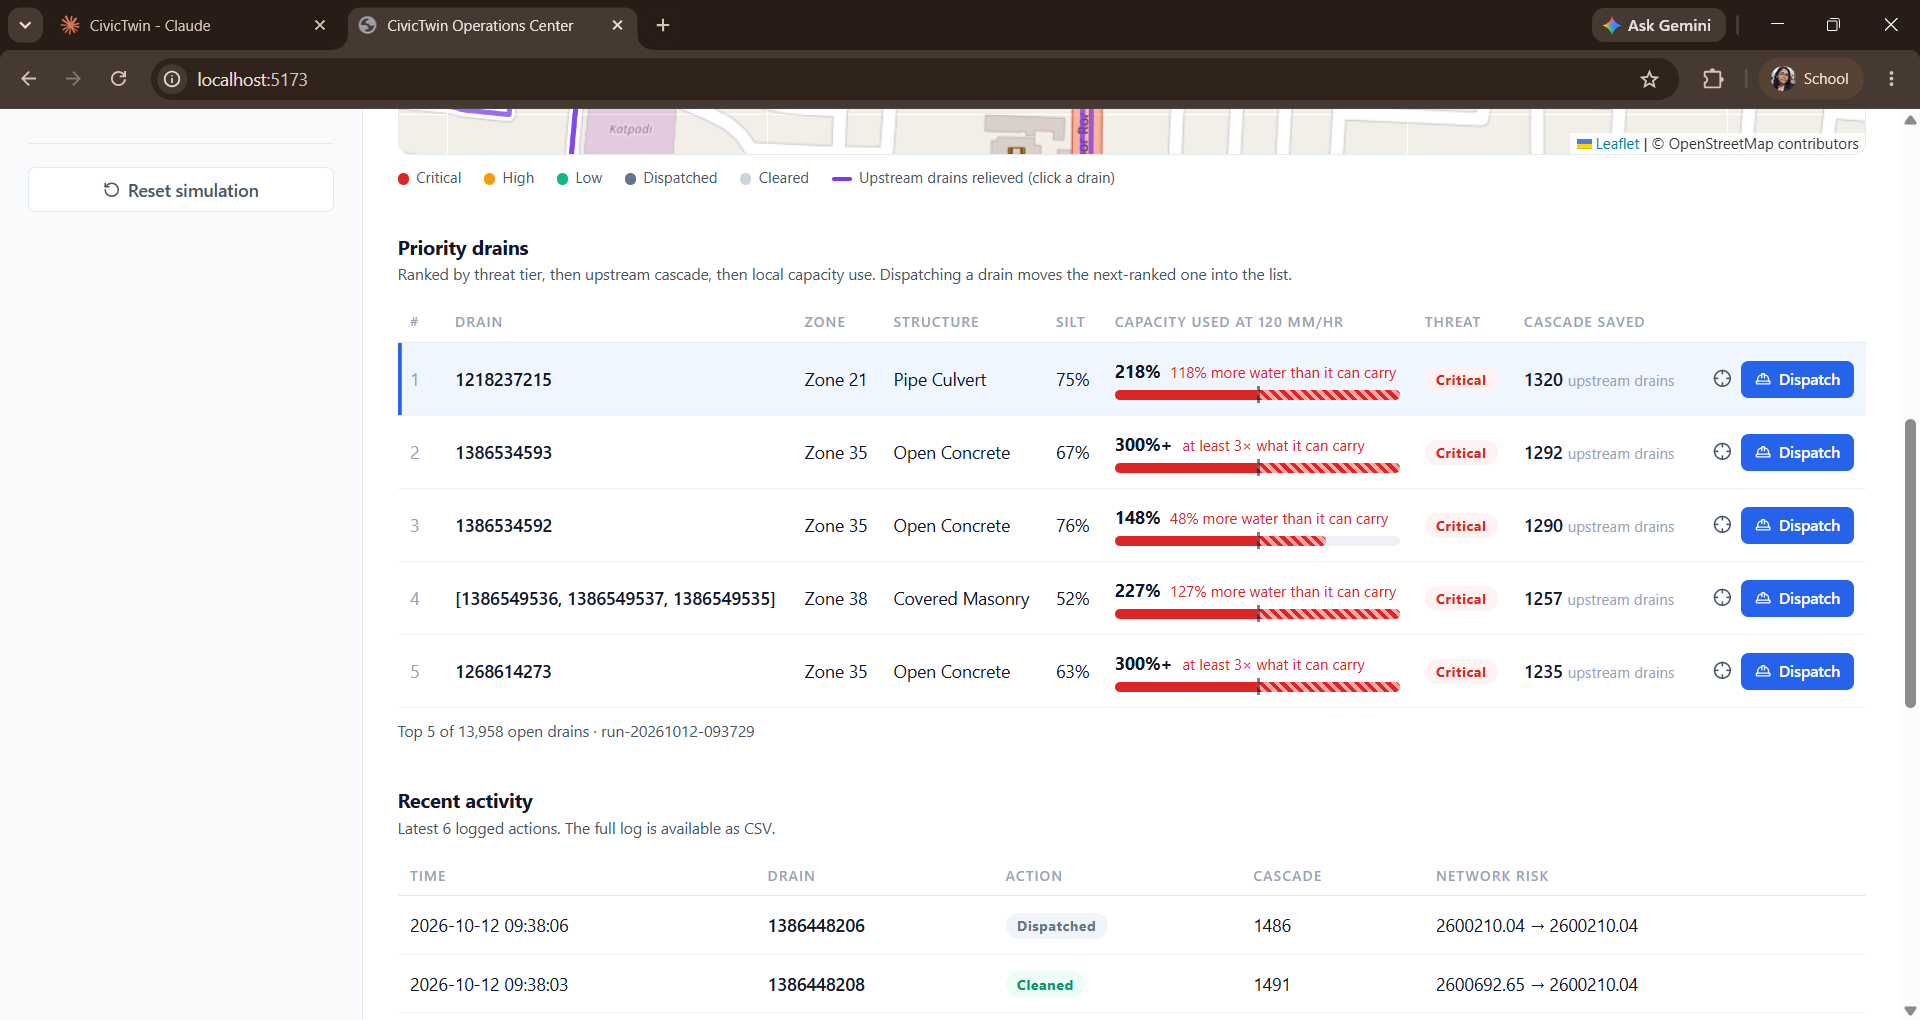
\includegraphics[width=0.98\textwidth]{figures/ui_priority_table.png}
\caption{Priority Dispatch Table with Real-Time Capacity Surcharge Metrics}
\label{fig:ui_table}
\end{figure}

The table displays the top-$k$ urgent conduit recommendations ranked by the active strategy:
\begin{itemize}
    \item \textbf{Rank (\#):} Ordinal dispatch rank (1 to 5).
    \item \textbf{Drain Segment ID:} The unique OpenStreetMap way identifier (e.g., \texttt{1218237215}, \texttt{1386534593}). For joined multi-way conduits, the composite ID tuple is displayed.
    \item \textbf{Zone:} Administrative cluster number (e.g., Zone 21, Zone 35, Zone 38).
    \item \textbf{Structure:} Physical conduit construction typology (Pipe Culvert, Open Concrete, Covered Masonry).
    \item \textbf{Silt:} Baseline surveyed sediment blockage (e.g., 75\%, 67\%, 76\%).
    \item \textbf{Capacity Used at Rainfall Intensity:} An intuitive horizontal bar graphic with a vertical marker at 100\% and diagonal striped warning patterns illustrating excess surcharge (e.g., \textit{``218\% · 118\% more water than it can carry''}, or \textit{``300\%+ · at least $3\times$ what it can carry''}).
    \item \textbf{Threat Tier:} Badge indicating categorical risk (Critical).
    \item \textbf{Cascade Saved:} Upstream relief potential (e.g., \textit{``1,320 upstream drains''}, \textit{``1,292 upstream drains''}), providing immediate transparent rationale for the ranking.
    \item \textbf{Dispatch Button:} Interactive button that assigns the conduit to a field desilting crew.
\end{itemize}

Clicking \textbf{Dispatch} immediately transitions the segment to \texttt{IN\_PROGRESS}, moves it into the Active Queue on the sidebar, and backfills the next highest-ranked open conduit from the network into the priority list.

\section{Field Work Order Lifecycle and Operational Audit Trails}
Figure~\ref{fig:ui_logs} illustrates the lower section of the dashboard, encompassing the Recent Activity Audit Log, the Administrative Interpretation Guide, and metadata specifications.

\begin{figure}[h!]
\centering
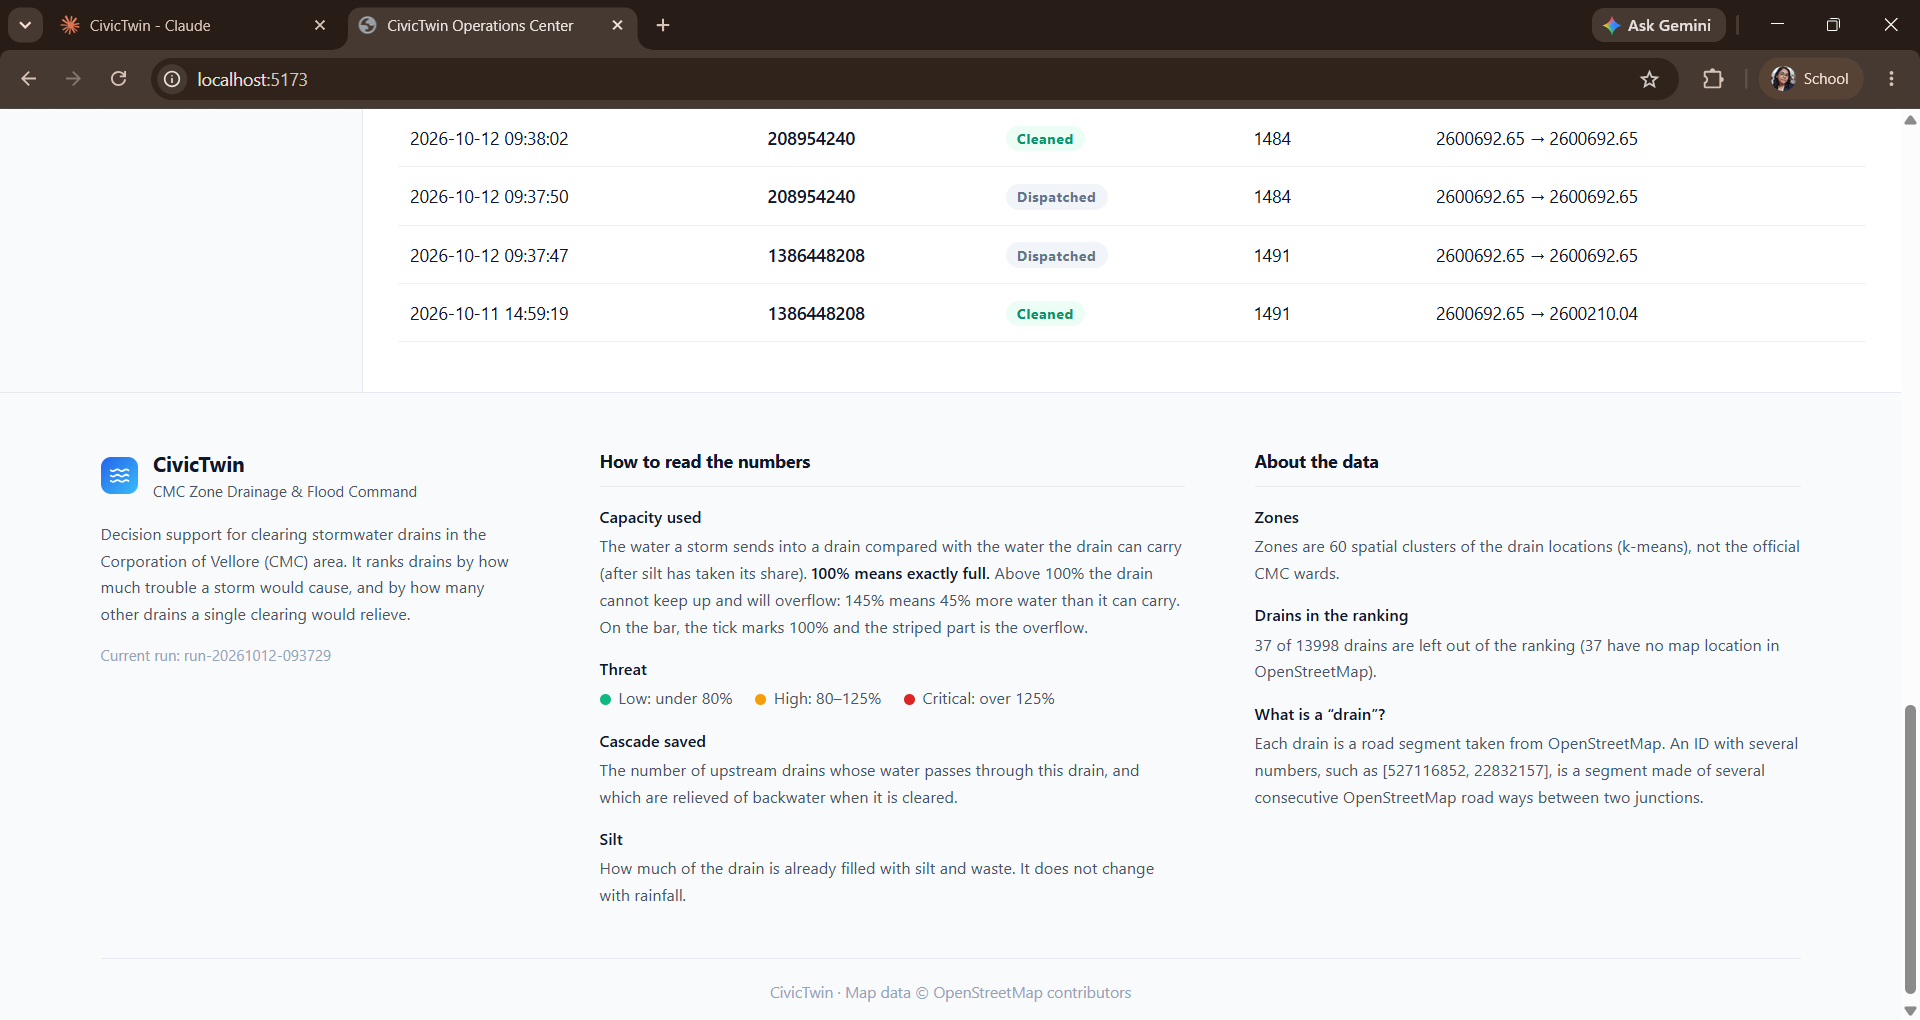
\includegraphics[width=0.98\textwidth]{figures/ui_logs_and_guide.png}
\caption{Recent Operational Activity Audit Log and Administrative Guide}
\label{fig:ui_logs}
\end{figure}

The \textbf{Recent Activity Log} records every action taken during the operational session:
\begin{itemize}
    \item \textbf{Timestamp:} Exact date and time down to the second (e.g., \texttt{2026-10-12 09:38:06}).
    \item \textbf{Drain Segment ID:} Conduit operated upon.
    \item \textbf{Action Badge:} Color-coded badge (\texttt{Dispatched} in light blue, \texttt{Cleaned} in light green, or \texttt{Survey Update}).
    \item \textbf{Cascade Relieved:} Upstream tributary count relieved by the intervention (e.g., 1,486, 1,491 drains).
    \item \textbf{Network Risk Delta:} Quantitative exposure reduction before and after the action (e.g., $2{,}600{,}692.65 \rightarrow 2{,}600{,}210.04$, capturing an immediate systemic relief of 482.61 points).
\end{itemize}

The \textbf{Download History CSV} button on the header allows municipal supervisors to export the entire audit trail into spreadsheet software for administrative review and contractor invoicing. The \textbf{Reset Simulation} button enables engineers to reset the engine state back to initial survey conditions, facilitating repeatable storm contingency drills.
